\subsection{Propriedade}
Assim como a comparação com a programação estruturada abordando o que é um
método, seguindo a mesma analogia, uma propriedade (também conhecida como
atributo, variável membro ou ainda variável de instância) pode ser considerada
como os dados que um objeto possuí, descrevendo desta forma, as características
que a ele pertencem \cite{programmingPhp}.

Sendo assim, os atributos são variáveis que estão definidas dentro de uma
classe, deste modo, geralmente são acessados através de uma interface de acesso,
pois não estão visíveis para que outros objetos manipulem os dados diretamente,
se isto ocorresse, poderia comprometer a segurança da informação e também o
conceito de que cada objeto possuí uma finalidade.

Então, uma propriedade (pensando na classe carro) poderia ser uma característica
que um carro possuí no mundo real. Portanto, poderíamos levantar de acordo com
o nosso conhecimento rapidamente os seguintes parâmetros que definem um carro:
cor, quantidade de portas, possuí direção hidráulica, etc.

\begin{figure}[h!tb]
	\caption{Criação de duas propriedade para a Classe Carro implementadas na
	linguagem PHP}
	\label{fig:propriedade}

	\centering
	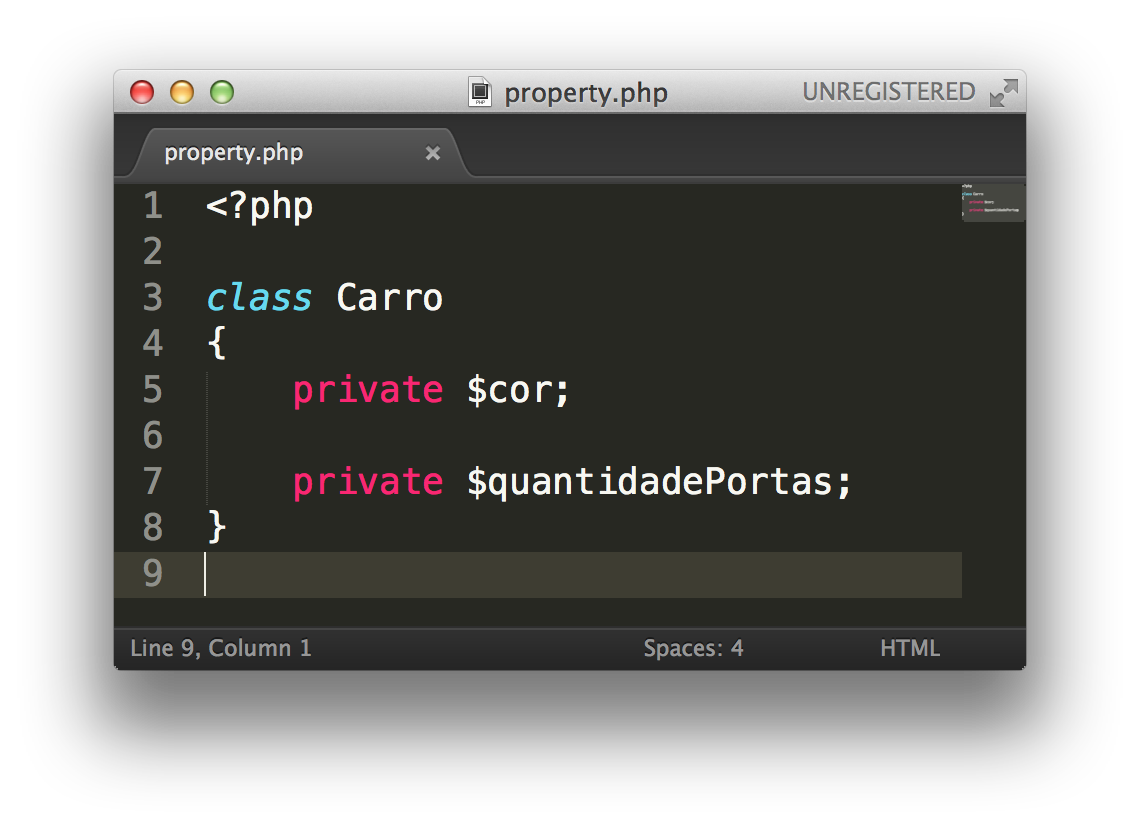
\includegraphics[width=0.75\textwidth]{images/property.png}

	\centering
	\footnotesize Fonte: \fonteOAutor
\end{figure}

\FloatBarrier 	% Este comando impede que as imagens
				% flutuem a partir deste ponto no seu documento

Por conseguinte, veremos abaixo uma análise da figura \ref{fig:propriedade}:

\begin{enumerate}[a)]
    \item linha 1: temos o início da execução de um bloco de código PHP;
    \item linha 3: definimos uma classe chamada \textit{Carro};
    \item linha 5: definimos uma palavra reservada chamada
    \textit{private} que se refere a visibilidade da propriedade no contexto  de
    um conjunto de objetos (veremos mais detalhes sobre a visibilidade adiante)
    e, em seguida, é definido o nome de uma variável, que neste caso chama-se
    \textit{\$cor};
    \item linha 7: é definida uma segunda propriedade para a classe
    carro chamada de \textit{\$quantidadePortas};
    \item linha 8: definimos onde termina o bloco que compreende a
    classe \textit{Carro}.
\end{enumerate}

\subsubsubsection{Propriedade Estática}

Como vimos anteriormente, as classes são formadas por variáveis de instância e
métodos. Entretanto, as variáveis que forem declaradas com a palavra reservada
static, serão compartilhadas por toda a classe. Por conta disto, as variáveis
que assim forem definidas, recebem o nome de variáveis estáticas ou ainda
propriedades estáticas \cite{learningJava}.

Veremos abaixo um exemplo de propriedade estática utilizando a linguagem PHP:
